\documentclass[11pt, oneside, a4paper]{book}

% ----------------------------------------------------------------------------
% Preamble
% ----------------------------------------------------------------------------

% Package to manage page layout
\usepackage[a4paper, top=25.4mm, bottom=25.4mm, right=25.4mm, left=40mm]{geometry}

% Line spacing: single=1 one-and-a-half=1.3 double=1.6
\linespread{1.3}

% Package to manage appendix
\usepackage[toc]{appendix}

% Package to insert empty lines between paragraphs
\usepackage[parfill]{parskip}

% Package to manage headers and footers
\usepackage{fancyhdr}

% define two header-footer styles
% 'normal' for most pages
\fancypagestyle{normal}{
\fancyhf{}
\fancyhead[L]{\slshape \leftmark} %chapter
\fancyhead[R]{\thepage} %footer
\renewcommand{\headrulewidth}{1pt}
}
% 'chapterstyle' for start of chapters (no chapter in header)
\fancypagestyle{chapterstyle}{
    \fancyhf{}
    \fancyhead[R]{\thepage}
    \renewcommand{\headrulewidth}{0pt}% Line at the header invisible
}

% Package to automatically change headerfooter style at start of chapters
\usepackage{etoolbox}
\patchcmd{\chapter}{\thispagestyle{plain}}{\thispagestyle{chapterstyle}}{}{}


% Package to get hyperrlinks
\usepackage{hyperref}

% Mathematics packages
\usepackage{amsmath}
\usepackage{amssymb}
\usepackage{mathtools}

% A package to include graphics files (jpg, png, eps, pdf etc...)
\usepackage{graphicx}

% A package that gives more control for bibliographies than the default
\usepackage[backend=biber,
			maxcitenames=2,
			maxbibnames=99,
			doi=false,
			url=false,
			bibstyle=apa,
			firstinits,
			uniquename=init,
			style=authoryear
            ]{biblatex}
\addbibresource{bibliography.bib}


% Package to add features for tables
\usepackage{multirow}
\usepackage{booktabs}
\setlength{\heavyrulewidth}{1.5pt}
\setlength{\abovetopsep}{4pt}

% Package to allow sub-figures
\usepackage{subcaption}


% A package to generate latin. You do not need this: I am just using it to get
% random text.
\usepackage{lipsum}

\usepackage{standalone}
\usepackage{tikz}
\usetikzlibrary{er,positioning, calc, patterns}
\usetikzlibrary{decorations.pathreplacing}
% ----------------------------------------------------------------------------
% The actual report
% ----------------------------------------------------------------------------

\begin{document}

\newgeometry{a4paper, top=25.4mm, bottom=25.4mm, right=25.4mm, left=25.4mm}
\begin{titlepage}
	\begin{center}
		\vspace*{1cm}
		\vspace{10pt}

		\hrule
		\vspace{10pt}
		\huge
		\textsc{Understanding responses to environments for the Prisoner's Dilemma:
		A meta analysis, multidimensional optimisation and machine learning approach}
		\vspace{15pt}
		\hrule
		
		\vspace{2cm}

		
\includegraphics[width=40mm]{cardiff_logo.jpg}
		\vspace{1cm}

		\LARGE
		Nikoleta E. Glynatsi
		
		\vspace{2cm}
		\large
		Submitted in partial fulfillment of\\ the requirements for the degree of\\[0.35em] Doctor of Philosophy. \\
		\vspace{1cm}
		May 2020

	\end{center}
\end{titlepage}
\restoregeometry

\frontmatter
\pagestyle{chapterstyle} %set header-footer style for front matter
\chapter{Executive Summary}

\lipsum[1-9]
\chapter{Acknowledgements}

First and foremost, I would like to express my greatest and utmost gratitude to
my tolerant and supportive supervisor, Dr Vincent Knight, whose guidance,
encouragement and jokes have been invaluable throughout my PhD. I am extremely
grateful for our long research meetings, our friendly chats that concluded with
me spoiling a movie/show for you, and our academic trips around the world.

I would also like to thank Dr Jonathan Gillard for his advice through parts of
this work and Dr Marc Harper for his input and commentary in the narrative on
the meta tournaments research.

On a more personal note, I would like to thank my family who have been a source
of great inspiration and motivation throughout life. They never questioned my
decisions and have supported me to the fullest. Except that time when my mother
disapproved of me travelling to New York alone.  I would like to express  my
sincere gratitude to my friends Nicki Verdeli, Kostas Soulanis and Chris
Athanasiou, for their continuous support and friendship throughout my years in
Cardiff. Their homemade meals, inspirational talks about not getting anxious and
competitive games of UNO have been vital in the completion of this PhD. 

I would also like to thank my colleagues Waleed Ali, Asyl Hawa, Geraint Palmer,
Chris Seaman, Lorenzo De Biase, Henry Wilde and Emily O'Riordan for their
company and endless coffee breaks. Finally, I would like to thank Mrs Joanna
Emery for making my academic journey in Cardiff University possible, and the
professional services staff of the School for Mathematics for their continuous
help the past four years with filling forms, booking rooms, resolving IT issues
and preparing coffee and biscuits.

\tableofcontents
\listoffigures
\listoftables
\chapter{Summary}

\lipsum[1-3]

\mainmatter
\pagestyle{normal} %set header-footer style rest of report


\chapter{Introduction}
\chapter{A systematic literature review of the Prisoner's Dilemma.}

    The Prisoner's Dilemma is a well known game used since the 1950's as a
    framework for studying the emergence of cooperation; a topic of continuing
    interest for mathematical, social, biological and ecological sciences. The
    iterated version of the game, the Iterated Prisoner's Dilemma, attracted
    attention in the 1980's after the publication of the ``The Evolution of
    Cooperation'' and has been a topic of pioneering research ever since. The
    aim of this paper is to provide a systematic literature review on Prisoner's
    Dilemma related research. This is achieved by reviewing selected pieces of
    work and partition the literature into five different sections with each
    reviewing a different aspect of research. The questions answered in this
    manuscript are (1) what are the research trends in the field (2) what are
    the already existing results within the field.

\section{Introduction}\label{section:introduction}

Based on the Darwinian principle of survival of the fittest cooperative behaviour
should not be favoured, however, cooperation is plentiful in nature.
A paradigm of understanding the emergence of these behaviours is
a particular two player non-cooperative game called the Prisoner's Dilemma (PD),
originally described in~\cite{Flood1958}.

In the PD each player has two choices, to either be selfless and cooperate or to
be selfish and defect. Each decision is made simultaneously and
independently. The utility of each player is influenced by its own behaviour,
and the behaviour of the opponent. Both players do better if they choose to
cooperate than if both choose to defect. However, a player has the temptation to
deviate as that player will receive a higher payoff than that of mutual
cooperation.
Players' payoffs are generally represented by (\ref{eq:the_pd_payoffs}). Both
players receive a reward for mutual cooperation, \(R\), and a payoff \(P\) for
mutual defection. A player that defects while the other cooperates receives a payoff of
\(T\), whereas the cooperator receives \(S\). The dilemma exists due
to constraints (\ref{eq:constrain_one}) and (\ref{eq:constrain_two}).

\begin{equation}\label{eq:the_pd_payoffs}
    \begin{pmatrix}
    R & S \\ T & P
    \end{pmatrix}
\end{equation}

\begin{equation}\label{eq:constrain_one}
    T > R > P > S
\end{equation}

\begin{equation}\label{eq:constrain_two}
    2R > T + S
\end{equation}

Another common representation of the payoff matrix is given by~(\ref{eq:the_pd_payoffs_with_cost}),
where \(b\) is the benefit of the altruistic behaviour and \(c\) it's its cost
(constraints (\ref{eq:constrain_one}) and (\ref{eq:constrain_two}) still hold).

\begin{equation}\label{eq:the_pd_payoffs_with_cost}
    \begin{pmatrix}
        b - c & c \\ b & 0
    \end{pmatrix}
\end{equation}

Constraints (\ref{eq:constrain_one}-\ref{eq:constrain_two})
guarantee that it never benefits a player to cooperate, indeed mutual
defection is a Nash equilibrium. However, when the game is studied in a manner
where prior outcome matters, defecting is no longer necessarily the dominant
choice.

The repeated form of the game is called the Iterated Prisoner's Dilemma (IPD)
and theoretical works have shown that cooperation can emerge once players
interact repeatedly. Arguably, the most important of these works is Robert
Axelrod's ``The Evolution of Cooperation''~\cite{Axelrod1984}. In his book
Axelrod reports on a series of computer tournaments he organised. In these
tournaments academics from several fields were invited to design computer
strategies to compete. Axelrod's work showed that greedy
strategies did very poorly in the long run whereas altruistic strategies did
better. ``The Evolution of Cooperation'' is considered a milestone in the field
but it is not the only one. On the contrary, the PD has attracted attention ever
since the game's origins.

This manuscript presents a qualitative description of selected pieces
of work. These have been separated into five sections, each
reviewing a different aspect of research. The topics reviewed at each section
are the following:

\begin{itemize}
    \item section~\ref{section:origin}, \textbf{Origins of the Prisoner's
    Dilemma}.
    \item section~\ref{section:intelligent_design}, \textbf{Axelrod's
    tournaments and intelligent design of strategies}.
    \item section~\ref{section:evolutionary_dynamics}, \textbf{Evolutionary dynamics}
    \item section~\ref{section:structured_strategies}, \textbf{Structured
    strategies and training}.
    \item section~\ref{section:software}, \textbf{Software}.
\end{itemize}

The aim of this work is to provide a concrete summary of the existing literature
on the PD. This is done to provide a review which will allow the research
community to understand overall trends in the field, and already existing
results.

\section{Origins of the prisoner's dilemma}\label{section:origin}

The origin of the PD goes back to the 1950s in early experiments conducted at
RAND~\cite{Flood1958} to test the applicability of games described
in~\cite{VonNeumann1944}. The game received its name later the same year.
According to~\cite{Tucker1983}, Albert W. Tucker (the PhD supervisor of John
Nash~\cite{Nash1951}), in an attempt to deliver the game with a story during a
talk described the players as prisoners and the game has been known as the
Prisoner's Dilemma ever since.

The early research on the IPD was limited. The only source of
experimental results was through human subject research where pairs of
participants simulated plays of the game. Human subject research had
disadvantages. Humans could behave randomly and in several experiments both the
size and the background of the individuals were different, thus comparing
results of two or more studies became difficult.

The main aim of these early research experiments was to understand how
conditions such as the gender of the participants~\cite{Evans1966, Lutzker1961,
Mack1971}, the physical distance between the participants~\cite{Sensenig1972}, the
effect of their opening moves~\cite{Tedeschi1968} and even how the experimenter, by varying
the tone of their voice and facial expressions~\cite{Gallo1968}, could influence
the outcomes and subsequently the emergence of cooperation. An early figure that
sought out to understand several of these conditions was the mathematical
psychologist Anatol Rapoport. The results of his work are summarised
in \cite{rapoport1965}.

Rapoport was also interested in conceptualising strategies that could promote
international cooperation. Decades later he would submit the winning strategy
(Tit for Tat) of the first computer tournament, run by Robert Axelrod.
In the next section these tournaments,
and several strategies that were designed by researchers, such as Rapoport, are
introduced.

\section{Axelrod's tournaments and intelligently designed strategies}
\label{section:intelligent_design}

As discussed in Section~\ref{section:origin}, before 1980 a great deal of
research was done in the field, however, as described in~\cite{Axelrod2012}, the
political scientist Robert Axelrod believed that there was no clear answer to the
question of how to avoid conflict, or even how an individual should play the
game. Combining his interest in artificial intelligence and political science
Axelrod created a framework for exploring these questions using computer
tournaments. Axelrod asked researchers to design a strategy with the purpose of
wining an IPD tournament. This section covers Axelrod's original
tournaments as well as research that introduced new intelligently designed
strategies.

Axelrod's tournaments made the study of cooperation of critical interest. As
described in~\cite{Rapoport2015}, ``Axelrod's “new approach” has been extremely
successful and immensely influential in casting light on the conflict between an
individual and the collective rationality reflected in the choices of a
population whose members are unknown and its size unspecified, thereby opening a
new avenue of research''. In a collaboration with a colleague, Douglas Dion,
Axelrod in~\cite{Axelrod1988} summarized a number of works that were immediately
inspired from the ``Evolution of Cooperation'', and~\cite{Jurisic2012} gives a
review of tournaments that have been conducted since the originals.

The first reported computer tournament took place in 1980~\cite{Axelrod1980a}. A
total of 13 strategies were submitted, written in the programming languages
Fortran or Basic. Each competed in a 200 turn match against all 12 opponents,
itself and a player that played randomly (called \textbf{Random}). This type of
tournament is referred to as a round robin. The tournament was repeated 5 times
to get a more stable estimate of the scores for each pair of play.
Each participant knew the exact number of turns and had access to the full
history of each match. Furthermore, Axelrod performed a preliminary tournament
and the results were known to the participants. This preliminary tournament is
mentioned in~\cite{Axelrod1980a} but no details were given. The payoff values
used for equation~(\ref{eq:the_pd_payoffs}) were \(R=3, P=1, T=5\) and \(S=0\).
These values are commonly used in the literature and unless specified will be
the values used in the rest of the works described here.

The winner of the tournament was determined by the total average score and not
by the number of matches won. The strategy that was announced the winner was the
strategy submitted by Rapoport, \textbf{Tit For Tat}. The success of Tit for Tat
came as a surprise. It was not only the simplest submitted strategy, it would
always cooperates on the first round and then mimic the opponent's previous
move, but it had also won the tournament even though it could never beat
any player it was interacting with.

In order to further test the results Axelrod performed a second tournament
in 1980~\cite{Axelrod1980b}. The second tournament received much more attention
and had a total of 62 entries. The participants knew the results of the previous
tournament and the rules were similar with only a few alterations. The
tournament was repeated 5 times and the length of each match was not known to
the participants. Axelrod intended to use a fixed probability (refereed to as
`shadow of the future'~\cite{Axelrod1988}) of the game ending on the next move.
However, 5 different number of turns were selected for each match 63, 77, 151,
308 and 401, such that the average length would be around 200 turns.

Nine of the original participants competed again in the second tournament. Two
strategies that remained the same were Tit For Tat and \textbf{Grudger}. Grudger
is a strategy that will cooperate as long as the opponent does not defect,
submitted by James W. Friedman. The name Grudger was give to the strategy
in~\cite{Li2014}, though the strategy goes by many names in the literature such
as, Spite~\cite{Beaufils1997}, Grim Trigger~\cite{Banks1990} and
Grim~\cite{Van2015}. New entries in the second tournament included \textbf{Tit
for Two Tats} submitted by John Maynard Smith and \textbf{KPavlovC}. KPavlovC,
is also known as Simpleton~\cite{rapoport1965}, introduced by Rapoport or just
Pavlov~\cite{Nowak1993}. The strategy is based on the fundamental behavioural
mechanism win-stay, lose-shift. Pavlov is heavily studied in the literature and
similarly to Tit for Tat it is used in tournaments today and has
had many variants trying to build upon it's success, for example
\textbf{PavlovD} and \textbf{Adaptive Pavlov}~\cite{Li2007}.

Despite the larger size of the second tournament none of the new entries managed
to outperform the simpler designed strategy. The winner was once again Tit for
Tat. Axelrod deduced the following guidelines for a strategy to perform well:

\begin{itemize}
    \item The strategy would start of by cooperating.
    \item It would forgive it's opponent after a defection.
    \item It would always be provoked by a defection no matter the history.
    \item It was simple.
\end{itemize}

The success of Tit for Tat, however, was not unquestionable. Several papers
showed that stochastic uncertainties severely undercut the effectiveness of
reciprocating strategies and such stochastic uncertainties have to be expected
in real life situations~\cite{Milinski1987}. For example, in~\cite{Molander1985}
it is
proven that in an environment where \textbf{noise} (a probability that a
player's move will be flipped) is introduced two strategies playing Tit for Tat
receive the same average payoff as two Random players.
Hammerstein, pointed out that if by mistake, one of two
Tit for Tat players makes a wrong move, this locks the two opponents into a
hopeless sequence of alternating defections and cooperations~\cite{Hammerstein1984}.

The poor performance of the strategy in noisy environments was also demonstrated
in tournaments. In~\cite{Bendor1991, Donninger1986} round robin
tournaments with noise were performed, and Tit For Tat did not win.
The authors concluded that to overcome the noise more generous strategies
than Tit For Tat were needed. They introduced the strategies \textbf{Nice and Forgiving}
and \textbf{OmegaTFT} respectively.

A second type of stochastic uncertainty is
misperception, where a player's action is made correctly but it is recorded
incorrectly by the opponent. In~\cite{Wu1995}, a strategy
called~\textbf{Contrite Tit for Tat} was introduced that was more successful than Tit for Tat
in such environments. The difference between the strategies was that Contrite
Tit for Tat was not so fast to retaliate against a defection.

Several works extended the reciprocity based approach which has led to new
strategies. For example Gradual~\cite{Beaufils1997} which was constructed to
have the same qualities as those of Tit for Tat except one,
\textbf{Gradual} had a memory of the game since the beginning of it. Gradual
recorded the number of defections by the opponent and punished them with a
growing number of defections. It would then enter a calming state in which it
would cooperates for two rounds. In a tournament of 12 strategies, including
both Tit for Tat and Pavlov, Gradual managed to outperformed them all. A
strategy with the same intuition as Gradual is \textbf{Adaptive Tit for
Tat}~\cite{tzafestas-2000a}. Adaptive Tit for Tat does not keep a permanent
count of past defections, it maintains a continually updated estimate of the
opponent’s behaviour, and uses this estimate to condition its future actions. In
the exact same tournament as in~\cite{Beaufils1997} with now 13 strategies Adaptive
Tit for Tat ranked first.

Another extension of strategies was that of teams of
strategies~\cite{J.P.Delahaye1993Lp, J.P.Delahaye1995LIeP, A.Rogers2007Ctpw}
that collude to increase one member's score. In 2004 Graham Kendall led the
Anniversary Iterated Prisoner's Dilemma Tournament with a total of 223 entries.
In this tournament participants were allowed to submit multiple strategies. A
team from the University of Southampton submitted a total of 60
strategies~\cite{A.Rogers2007Ctpw}. All these were strategies that had been
programmed with a recognition mechanism by default. Once the strategies
recognised one another, one would act as leader and the other as a follower. The
follower plays as a \textbf{Cooperator}, cooperates unconditionally and the
leader would play as a \textbf{Defector} gaining the highest achievable score.
The followers would defect unconditionally against other strategies to lower
their score and help the leader. The result was that Southampton had the top
three performers. Nick Jennings, who was part of the team, said that ``We
developed ways of looking at the Prisoner's Dilemma in a more realistic
environment and we devised a way for computer agents to recognise and collude
with one another despite the noise. Our solution beats the standard Tit For Tat
strategy"~\cite{southampton_blog}.

\subsection{Memory one Strategies}\label{section:memory_one}

A set of strategies that have received a lot of attention in
the literature are \textbf{memory one} strategies. In~\cite{nowak1989},
Nowak and Sigmund proposed a structure for studying simple strategies that
remembered only the previous turn, and moreover, only recorded the move of the
opponent. These are called \textbf{reactive} strategies and they can be
represented by using three parameters \((y, p_1, p_2)\), where \(y\) is the
probability to cooperate in the first move, and \(p_1\) and \(p_2\) the
conditional probabilities to cooperate, given that the opponent's last move was
a cooperation or a defection. For example Tit For Tat is a reactive strategy and
it can be written as \((1, 1, 0)\). Another reactive strategy well known in
the literature is \textbf{Generous Tit for Tat}~\cite{Nowak1992}.

In~\cite{Nowak1990}, Nowak and Sigmund extended
their work to include strategies which consider the entire history of the previous turn to make a decision.
These are called \textbf{memory one} strategies.
If only a single turn of the game is taken into account and depending on the
simultaneous moves of the two players there are only four possible states that
the players could be in. These are:

\begin{itemize}
    \item Both players cooperated, denoted as \(CC\).
    \item First player cooperated while the second one defected, denoted as \(CD\).
    \item First player defected while the second one cooperated, denoted as \(DC\).
    \item Both players defected, denoted as \(DD\).
\end{itemize}

Thus a memory one strategy can be denoted by the probabilities of cooperating
after each state and the probability of cooperating in the first round, \((y,
p_1, p_2, p_3, p_4)\). For example Pavlov's memory one representation is \((1,
1, 0, 0, 1)\).

Memory one strategies made an impact when a specific set of memory one
strategies were introduced called \textbf{Zero-determinant}
(ZD)~\cite{Press2012}. The American Mathematical Society's news section~\cite{hilbe2015}
stated that ``the world of game theory is currently on fire'' and in~\cite{Stewart2012}
it was stated that
``Press and Dyson have fundamentally changed the viewpoint on the Prisoner's Dilemma''.
ZD are a set of
extortionate strategies that can force a linear relationship between
the long-run scores of both themselves and the opponent, therefore ensuring that the
opponent will never do better than them.

Press and Dyson's suggested ZD strategies were the dominant family of strategies in the
IPD. Moreover, they argued that memory is not beneficial. In~\cite{Adami2013, Knight2017,
Hilbe2013, Hilbe2013b, hilbe2015, KnightHGC17, Knight2019, Lee2015, Stewart2012} the
effectiveness of ZD strategies is questioned. In~\cite{Adami2013}, it was shown that ZD
strategies are not evolutionary stable, and in~\cite{Stewart2012} a more
generous set of ZDs, the~\textbf{Generous ZD}, were shown to outperform the more
extortionate ZDs. Finally, in~\cite{Knight2017, KnightHGC17, Knight2019, Lee2015}, the `memory does not benefit a
strategy' statement was questioned. A set of more complex strategies, strategies
that take in account the entire history set of the game, were trained and proven
to be more stable than ZD strategies.

This section covered the original computer tournaments of Axelrod and
the early success of Tit For Tat in these tournaments. Though Tit For Tat was
considered to be the most robust basic strategy, reciprocity was found to not
be enough in environments with uncertainties. There are at least two properties,
that have been discussed in this section, for coping with such uncertainties;
generosity and contrition. Generosity is letting a percentage of defections go
unpunished, and contrition is lowering a strategy's readiness to defect
following an opponent's defection.

In the later part of this section a series of new strategies which were built on
the basic reciprocal approaches were presented, followed by the infamous memory
one strategies, the zero-determinant strategies. Though the ZDs can be proven to be robust
in pairwise interactions they were found to be lacking in evolutionary settings
and in computer tournaments. Evolutionary settings and the emergence
of cooperation under natural selection are covered in the next section.

\section{Evolutionary dynamics}\label{section:evolutionary_dynamics}

As yet, the emergence of cooperation has been discussed in the contexts of the
one shot PD game and the IPD round robin tournaments. In the PD it is
proven that cooperation will not emerge, furthermore, in a series of influential works
Axelrod demonstrated that reciprocal behaviour favours cooperation when
individuals interact repeatedly. But does natural selection favours cooperation?
Understanding the conditions under which natural selection can favour
cooperative behaviour is important in understanding social behaviour amongst
intelligent agents~\cite{Boyd1987}.

Imagine a mixed population of cooperators and defectors where every
time two individuals meet they play a game of PD. In such population the average
payoff for defectors is always higher than cooperators. Under natural selection
the frequency of defectors will steadily increase until cooperators become
extinct. Thus natural selection favours defection in the PD
(Figure~\ref{fig:natural_selection_diagram}). However, there are several mechanisms
that allow the emergence of cooperation in an evolutionary context which will be
covered in this section.

\begin{figure}[!hbtp]
    \centering
    \includestandalone{src/chapters/chapters-02/natural_selection}
    \caption{Natural selection favours defection in a mixed population of Cooperators
    and Defectors.}\label{fig:natural_selection_diagram}
\end{figure}

In the later sections of~\cite{Axelrod1980b}, Axelrod discusses an
ecological tournament that he performed using the 62 strategies of the second
tournament to understand the reproductive success of Tit for Tat. In his
ecological tournament the prevalence of each type of strategy in each round was
determined by that strategy's success in the previous round. The competition in
each round would become stronger as weaker performers were reduced and
eliminated. The ecological simulation concluded with a handful of nice
strategies dominating the population whilst exploitative strategies had died off
as weaker strategies were becoming extinct. This new result led Axelrod to
study the IPD in an evolutionary context based on several of the approaches
established by the biologist John M. Smith~\cite{Smith1974,
Smith1979, Smith1973}. John M. Smith was a fundamental figure in evolutionary game theory and a
participant of Axelrod's second tournament. Axelrod and the biologist William
Donald Hamilton wrote about the biological applications of the evolutionary
dynamics of the IPD~\cite{Axelrod1984} and won the
Newcomb-Cleveland prize of the American Association for the Advancement of
Science.

In Axelrod's model~\cite{axelrod1981} pairs of individuals from a
population played the IPD. The number of interactions between the pairs were
not fixed, but there was a probability defined as the importance of the future
of the game \(w\), where \(0 < w < 1\), that the pair would interact again. In
\cite{axelrod1981} it was shown that for
a sufficient high \(w\) Tit For Tat strategies
would become common and remain common because they were ``collectively stable".
Axelrod argued that collective stability implied evolutionary stability (ESS)
and that when a collectively stable strategy is common in a population and
individuals are paired randomly, no other rare strategy can invade. However,
Boyd and Lorderbaum in~\cite{Boyd1987} proved that if \(w\), the importance of the
future of the game, is large enough then no pure strategy is ESS because it can
always be invaded by any pair of other strategies. This was also independently
proven in~\cite{Pudaite1987}.

All these conclusions were made in populations where the individuals could all
interact with each other. In 1992, Nowak and May, considered a structured population
where an individual's interactions were limited to its neighbours.
More specifically, in~\cite{Nowak1992b} they explored how local interaction
alone can facilitate population wide cooperation in a one shot PD game. The two
deterministic strategies Defector and Cooperator, were placed onto a two
dimensional square array where the individuals could interact only with the
immediate neighbours. The number of immediate neighbours could be either,
fourth, six or eight, as shown in Figure~\ref{fig:topologies}, where each node
represents a player and the edges denote whether two players will interact. This
topology is refereed to as spatial topology. Each cell of the lattice is
occupied by a Cooperator or a Defector and at each generation step each cell owner
interacts with its immediate neighbours. The score of each player is calculated
as the sum of all the scores the player achieved at each generation. At the
start of the next generation, each lattice cell is occupied by the player with
the highest score among the previous owner and their immediate neighbours.

Local interactions proved that as long as small clusters of cooperators form, where
they can benefit from interactions with other cooperators while avoiding
interactions with defectors, global cooperation will continue. Thus, local
interactions proved that even for the PD cooperation can emerge. Moreover in
\cite{Ohtsuki2006}, whilst using the payoff
matrix~(\ref{eq:the_pd_payoffs_with_cost}), it was shown that cooperation will
evolve in a structured population as long as the benefit to cost ratio \(b / c\)
is higher than the number of neighbours. In~\cite{Perc2011}, graphs were a probability
of rewiring ones connections was considered were studied. The rewire could be with any
given node in the graphs and not just with immediate neighbours. Perc et al.
concluded that ``making new friends'' may be an important activity for the
successful evolution of cooperation, but also they must be selected
carefully and one should keep their number limited.

\begin{figure}[!hbtp]
\centering
    \begin{subfigure}{.25\textwidth}
        \includestandalone[width=\textwidth]{src/chapters/chapters-02/square_lattice}
    \end{subfigure}
    \begin{subfigure}{.25\textwidth}\centering
        \includestandalone[width=\textwidth]{src/chapters/chapters-02/hexagonal_lattice}
     \end{subfigure}
     \begin{subfigure}{.25\textwidth}\centering
        \includestandalone[width=\textwidth]{src/chapters/chapters-02/square_lattice_eight}
     \end{subfigure}
     \caption{Spatial neighbourhoods}\label{fig:topologies}
    \end{figure}

Another approach for increasing the likelihood of cooperation by increasing of
assortative interactions among cooperative agents, include partner identification
methods such as reputation~\cite{Janssen2006, Nowak1998, Suzuki2005},
communication tokens~\cite{Miller2002} and tags~\cite{Choi2006, Hales2000,
Miller2002, Riolo2001}.

In this section evolutionary dynamics and the emergence of cooperation were
reviewed. The following section focuses on strategy archetypes, training methods
and strategies obtained from training.

\section{Structured strategies and training}
\label{section:structured_strategies}

This section covers strategies that are different to that of intelligent design discussed
in Section~\ref{section:intelligent_design}. These are strategies that have
been \textbf{trained} using generic strategy archetypes. For example,
in~\cite{Axelrod1987} Axelrod decided to explore deterministic strategies that
took into account the last 3 turns of the game. As discussed in
Section~\ref{section:memory_one}, for each turn there are 4 possible outcomes,
\(CC, CD, DC, DD\), thus for 3 turns there are a total of
\(4\times4\times4=64\) possible combinations. Therefore, the strategy can be
defined by a series of 64 C's/D's, corresponding to each combination; this type
of strategy is called a lookup table.
This lookup table was then trained using a
genetic algorithm~\cite{Koza1997}. During the training process random changes are made to a
given lookup table. If the utility of the strategy has increased this
change is kept, otherwise not.

In 1996 John Miller considered finite state automata as an
archetype~\cite{Miller1996}, more specifically, Moore
machines~\cite{moore1956}. He used a genetic algorithm to train finite state
machines in environments with noise. Miller's results showed that even a small
difference in noise (from 1\% to 3\%) significantly changed the characteristics
of the evolving strategies. The strategies he introduced were \textbf{Punish
Twice}, \textbf{Punish Once for Two Tats} and \textbf{Punish Twice and Wait}.
In~\cite{Ashlock2006b} finite state automata and genetic algorithms were also
used to introduce new strategies. In a series of experiments where the size of
the population varied, there were two strategies frequently developed by the
training process and more over they were developed only after the evolution had
gone on for many generations. These were \textbf{Fortess3} and
\textbf{Fortess4}.
Following Miller's work in 1996, the first structured strategies based on neural
networks that had be trained using a genetic algorithm was introduced
in~\cite{Harrald1996} by Harrald and Fogel. Harrald and Fogel considered a
single layered neural network which had 6 inputs. These were the last 3 moves of
the player and the opponent, similar to~\cite{Axelrod1987}. Neural networks have
broadly been used to train IPD strategies since then with genetic
algorithms~\cite{Ashlock2006a, Chong2005, Marks1999} and particle swarm
optimization~\cite{Franken2005}.

In~\cite{Knight2017, KnightHGC17} both genetic algorithm and particle swarm
optimization were used to introduce a series of structured strategies based on
lookup tables, finite state machines, neural networks, hidden Markov
models~\cite{eddy1996} and Gambler. Hidden Markov models, are a stochastic
variant of a finite state machine and Gamblers are stochastic variants of lookup
tables. The structured strategies that arised from the training were put up
against a large number of strategies in (1) a Moran process, which is an
evolutionary model of invasion and resistance across time during which high
performing individuals are more likely to be replicated and (2)
a round robin tournament. In a round robin tournament which was simulated using the
software~\cite{axelrodproject} and the 200 strategies implemented within the
software, the top spots were dominated by the trained strategies of all the
archetypes. The top three strategies were \textbf{Evolved
LookUp 2 2 2}, \textbf{Evolved HMM 5} and \textbf{Evolved FSM 16}.

In~\cite{KnightHGC17} it was demonstrated that these trained strategies
would overtake the population in a Moran process. The strategies evolved an ability
to recognise themselves by using a handshake. This recognition mechanism allowed the strategies
to resist invasion by increasing the interactions between themselves, an approach
similar to the one described in Section~\ref{section:evolutionary_dynamics}.

Throughout the different methods of training that have been discussed in this
section, a spectrum of structured strategies can be found. Differentiating
between strategies is not always straightforward. It is not obvious looking at a
finite state diagram how a machine will behave, and many different machines, or
neural networks can represent the same strategy. For example
Figure~\ref{fig:machine_tft} shows two finite automata and both are a
representation of Tit for Tat.

\begin{figure}[!hbtp]
    \begin{subfigure}{.45\textwidth}\centering
        \includestandalone[height=.1\textheight]{src/chapters/chapters-02/tit_for_tat_fsm_one}
        \caption{Tit for Tat as a finite state machine with 1 state.}\label{fig:representation_a}
    \end{subfigure}
    \begin{subfigure}{.45\textwidth}\centering
        \includestandalone[height=.1\textheight]{src/chapters/chapters-02/tit_for_tat_fsm}
        \caption{Tit for Tat as a finite state machine with 2 states.}\label{fig:representation_b}
     \end{subfigure}
     \caption{Finite state machine representations of Tit for Tat. A machine
     consists of transition arrows associated with the states. Each arrow is
     labelled with \(A/R\) where \(A\) is the opponent's last action and \(R\)
     is the player's response. Finite state machines consist of a set of
     internal states. In (a) Tit for Tat finite state
     machine consists of 1 state and in (b) of 2.}\label{fig:machine_tft}
\end{figure}

To allow for identification of similar strategies a method called
fingerprinting was introduced in~\cite{Ashlock2005}. The method of fingerprinting is a
technique for generating a functional signature for a
strategy~\cite{Ashlock2008}. This is achieved by computing the score of a
strategy against a spectrum of opponents. The basic method is to play the
strategy against a probe strategy with varying noise parameters.
In~\cite{Ashlock2005} Tit for Tat is used as the probe strategy. In
Figure~\ref{fig:fingerprinting} an example of Pavlov's fingerprint is given.
Fingerprinting has been studied in depth in~\cite{Ashlock2008, Ashlock2009,
Ashlock2010, Ashlock2006a}. Another type of fingerprinting is the
transitive fingerprint~\cite{axelrodproject}.
The method represents the cooperation rate of a strategy against a set of opponents
over a number of turns. An example of a transitive fingerprint is given in
Figure~\ref{fig:transitive_fingerprinting}.

\begin{figure}[!hbtp]
    \centering
    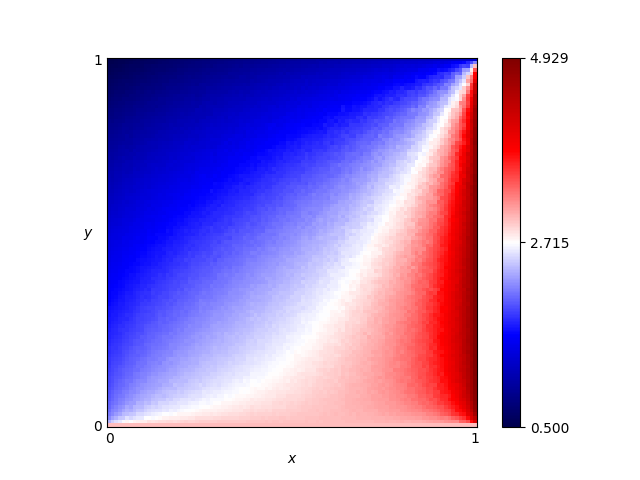
\includegraphics[height=.3\textheight]{src/chapters/chapters-02/Win-Stay_Lose-Shift.png}
    \caption{Pavlov fingerprinting with Tit for Tat used as the probe strategy.
    Figure was generated using~\cite{axelrodproject}.}
    \label{fig:fingerprinting}
\end{figure}

\begin{figure}[!hbtp]
    \centering
    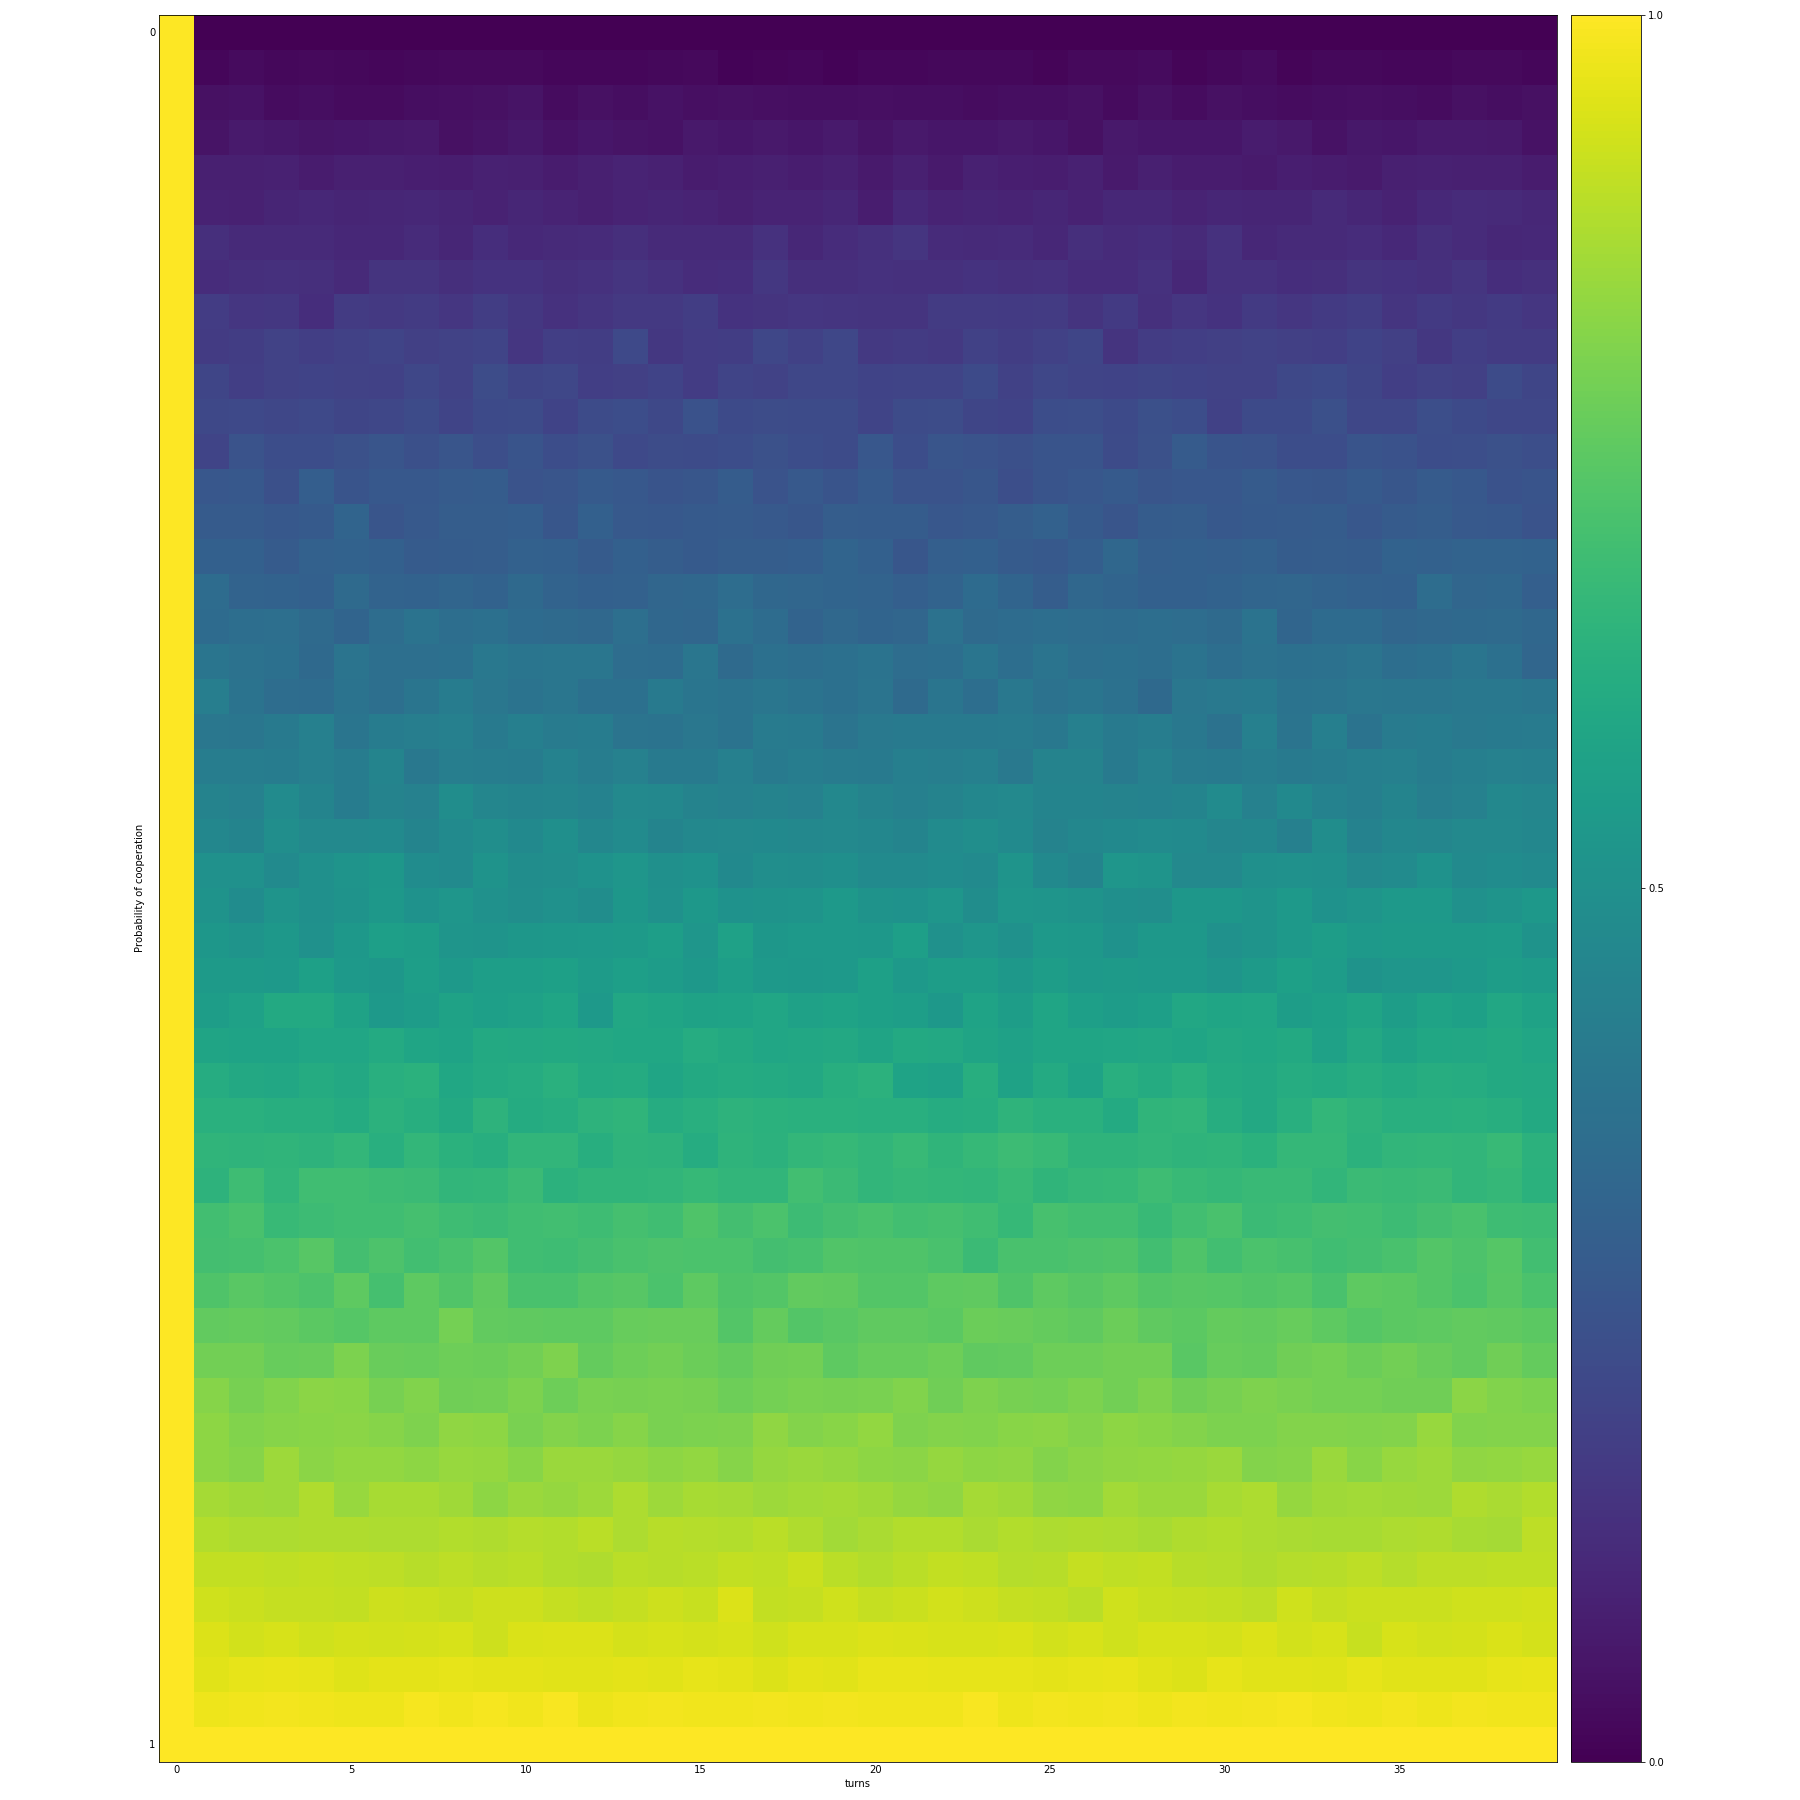
\includegraphics[height=.3\textheight]{src/chapters/chapters-02/Tit_for_Tat_fingerprint.png}
    \caption{Transitive fingerprint of Tit for Tat against a set of 50 random opponents.}
    \label{fig:transitive_fingerprinting}
\end{figure}

This section covered structured strategies and training methods. In the following
section software that has been developed with main aim simulating the IPD
is presented.

\section{Software}\label{section:software}

The research of the IPD heavily relies on software.
This is to be expected as computer tournaments have become the main
means of simulating the interactions in an IPD game.
Many academic fields suffer from lack of source code availability and the IPD
is not an exception. Several of the tournaments that have been discussed so far were generated
using computer code, though not all of the source code is available.
The code for Axelrod's original tournament is known to be lost and
moreover for the second tournament the only source code available is the code
for the 62 strategies (found on Axelrod's personal website~\cite{fortan_code}).

Several projects, however, are open, available and have been used as research
tools or educational platforms over the years. Two research tools~\cite{prison,
axelrodproject} and two educational tools~\cite{pd_trust, pd_game} are briefly
mentioned here. Both~\cite{prison, axelrodproject} are open
source projects.
The ``Game of Trust"~\cite{pd_trust} is an on-line, graphical user interface
educational platform for learning the basics of game theory, the IPD
and the notion of strategies. It attracted a lot of attention
due to being ``well-presented with scribble-y hand drawn
characters''~\cite{trust_blogb} and ``a whole heap of fun''~\cite{trust_bloga}.
Finally~\cite{pd_game} is a personal project written in PHP. It is a graphical user
interface that offers a big collection of strategies and allows the user to try
several matches and tournament configurations.

PRISON~\cite{prison} is written in the programming
language Java and a preliminary version was launched on 1998. It was used by its
authors in several publications, such as~\cite{Beaufils1997}, which introduced
Gradual, and~\cite{Beaufils1988}. The project includes a good number of
strategies from the literature but unfortunately the last update of the project
dates back to 2004. Axelrod-Python~\cite{axelrodproject} is a software used
by~\cite{Knight2017,KnightHGC17, Goodman2018, Wang2017}. It is written in the
programming language Python following best practice approaches~\cite{Aberdour2007,
Benureau2018} and contains the
largest collection of strategies, known to the author. The strategy list of
the project has been cited by publications~\cite{Anastassacos2018, Hayes2017,
Neumann2018}.

\section{Conclusion}

This manuscript presented a literature review on the Iterated Prisoner's
Dilemma. The opening sections focused on research trends and published works of
the field, followed by a presentation of research and educational software.
More specifically, Section~\ref{section:origin}
covered the early years of research. This was when simulating turns of the game
was only possible with human subject research.
Following the early years, the pioneering tournaments of Axelord were introduced in
Section~\ref{section:intelligent_design}. Axelrod's work offered the field an
agent based game theoretic framework to study the IPD.
In his original papers he asked researchers to design strategies to test their
performance with the new framework. The winning strategy of both his tournaments
was Tit for Tat. The strategy however came with limitations which were explored
by other researchers, and new intelligently designed strategies were introduced in
order to surpass Tit for Tat with some contributions such as Pavlov and Gradual.

Soon researchers came to realise that strategies should not just do well in a tournament setting
but should also be evolutionary robust. Evolutionary dynamic methods were
applied to many works in the field, and factors under which cooperation
emerges were explored, as described in Section~\ref{section:evolutionary_dynamics}.
This was not done only for unstructured populations, where all strategies
in the population can interact with each other, but also in population where
interactions were limited to only strategies that were close to each other.
In such topologies it was proven that even in the one shot game, cooperation can
indeed emerge.

Evolutionary approaches can offer many insights in the study of the PD. In
evolutionary settings strategies can learn to adapt and take over population by
adjusting their actions; such algorithms can be applied so that evolutionarily
robust strategies can emerge. Algorithms and structures used to train strategies
in the literature were covered in Section~\ref{section:structured_strategies}.
From these training methods several strategies are found,
and to be able to differentiate between them fingerprinting was
introduced. The research of best play and cooperation has been going on since
the 1950s, and for simulating the game software has been developed along the
way. This software has been briefly discussed
in Section~\ref{section:software}.

The study of the PD is still an ongoing field research where new variants and
new structures of strategies are
continuously being explored~\cite{Ohtsuki2018}. The game now serves as a model
in a wide range of applications, for example in medicine and the study of cancer
cells~\cite{archetti2018, Kaznatchee2017}, as well as in social situations and
how they can be driven by rewards~\cite{Dridi2018}. New research is still ongoing
for example in evolutionarily dynamics on graphs~\cite{Allen2017, hathcock2018,
Liu2017}.

% \newpage
% \bibliographystyle{plain}
% \bibliography{bibliography.bib}
% \input{chapters/chapter3.tex}
% \input{chapters/chapter4.tex}



\addcontentsline{toc}{chapter}{References}
\printbibliography[title=References]

\begin{appendices}
% \chapter{Centrality measures distributions}

\section{Distributions for \(G\) and \(\bar{G}\)}

Betweeness and closeness centralities distributions for \(G\) and \(\bar{G}\).

\begin{figure}[!hbtp]
    \centering
    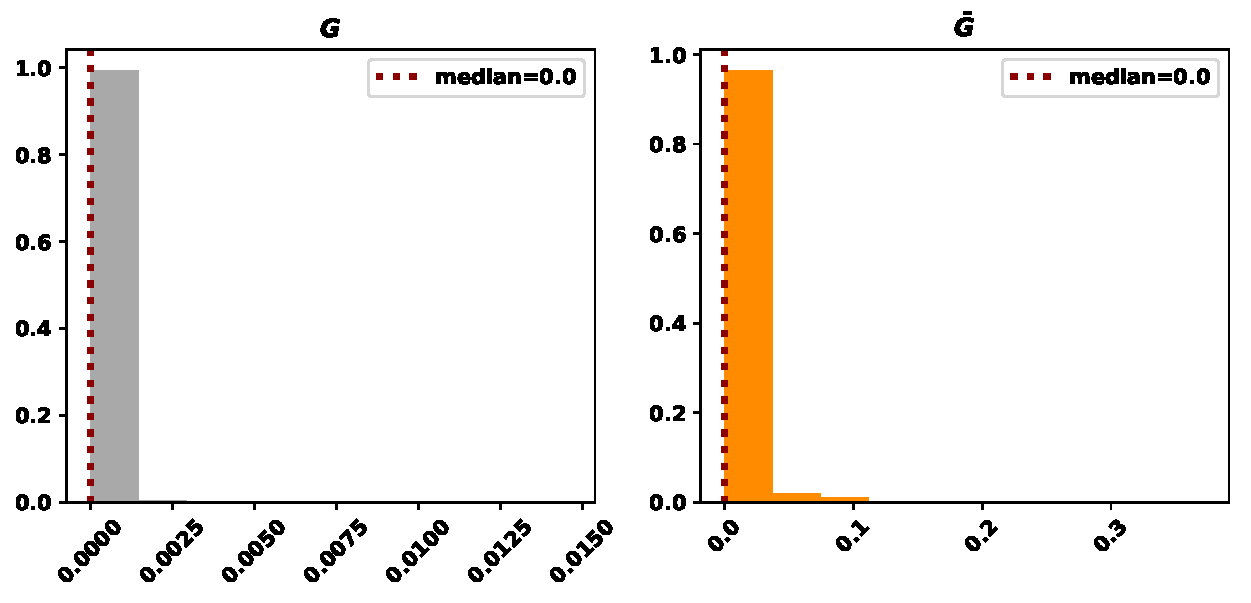
\includegraphics[width=.8\textwidth]{src/chapters/03/paper/bibliometric-study-of-the-prisoners-dilemma/assets/images/pd_betweeness_centralities.pdf}
    \caption{Distributions of betweenness centrality in \(G\) and \(\bar{G}\)}
    \label{fig:bc_distributions}
\end{figure}

\begin{figure}[!hbtp]
    \centering
    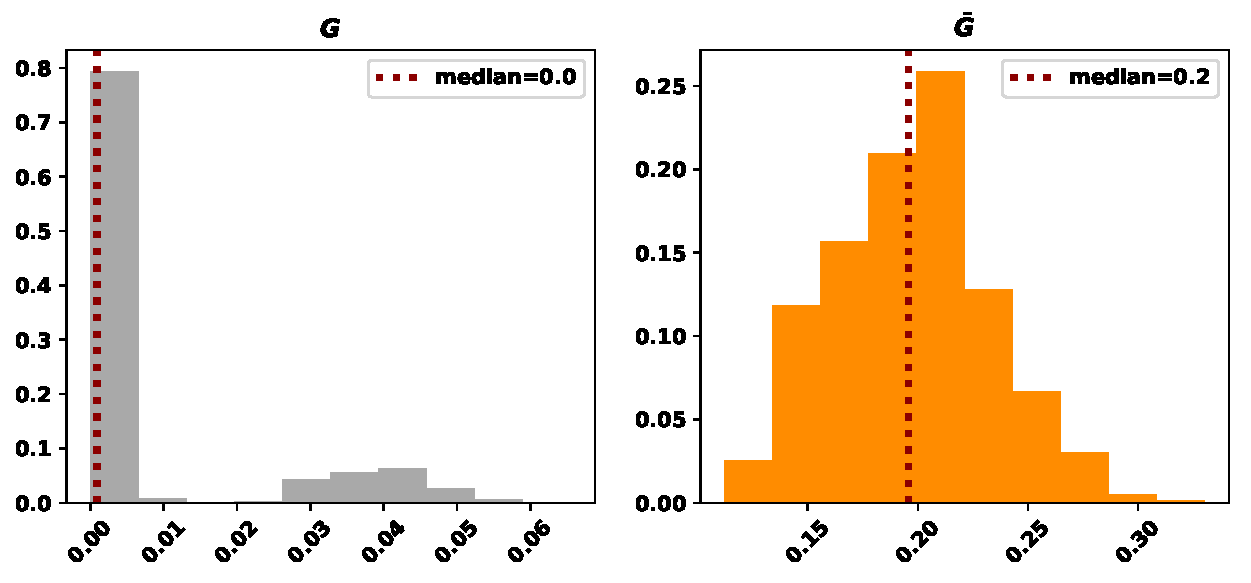
\includegraphics[width=.8\textwidth]{src/chapters/03/paper/bibliometric-study-of-the-prisoners-dilemma/assets/images/pd_closeness_centralities.pdf}
    \caption{Distributions of closeness centrality in \(G\) and \(\bar{G}\)}
    \label{fig:cc_distributions}
\end{figure}

\section{Distributions for topic networks}\label{appendix:distributions}

Betweeness and closeness centralities distributions for graphs of topics A to E.

\begin{figure}[!hbtp]
    \centering
    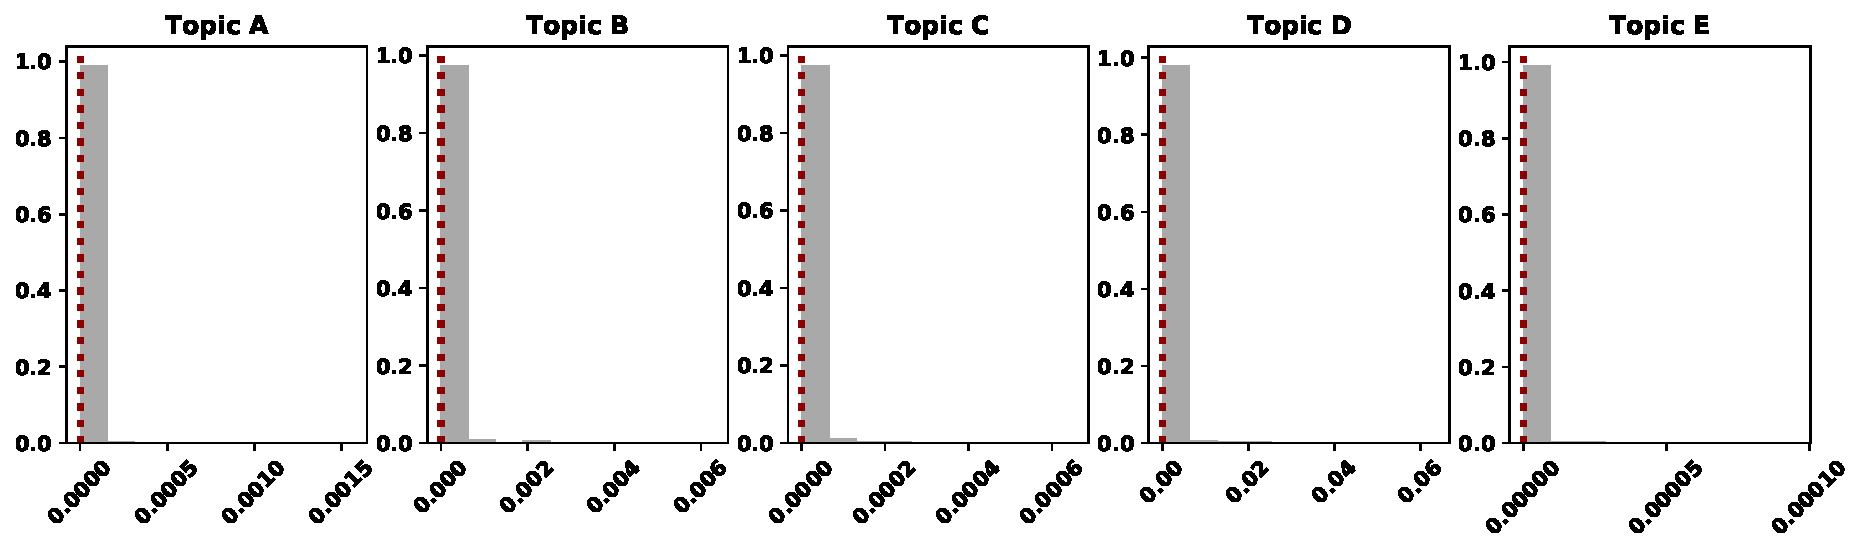
\includegraphics[width=\textwidth]{src/chapters/03/paper/bibliometric-study-of-the-prisoners-dilemma/assets/images/topics_betweeness_distributions.pdf}
    \caption{Distributions of betweenness centrality in topics' networks.}
    \label{fig:bc_distributions_topics}
\end{figure}

\begin{figure}[!hbtp]
    \centering
    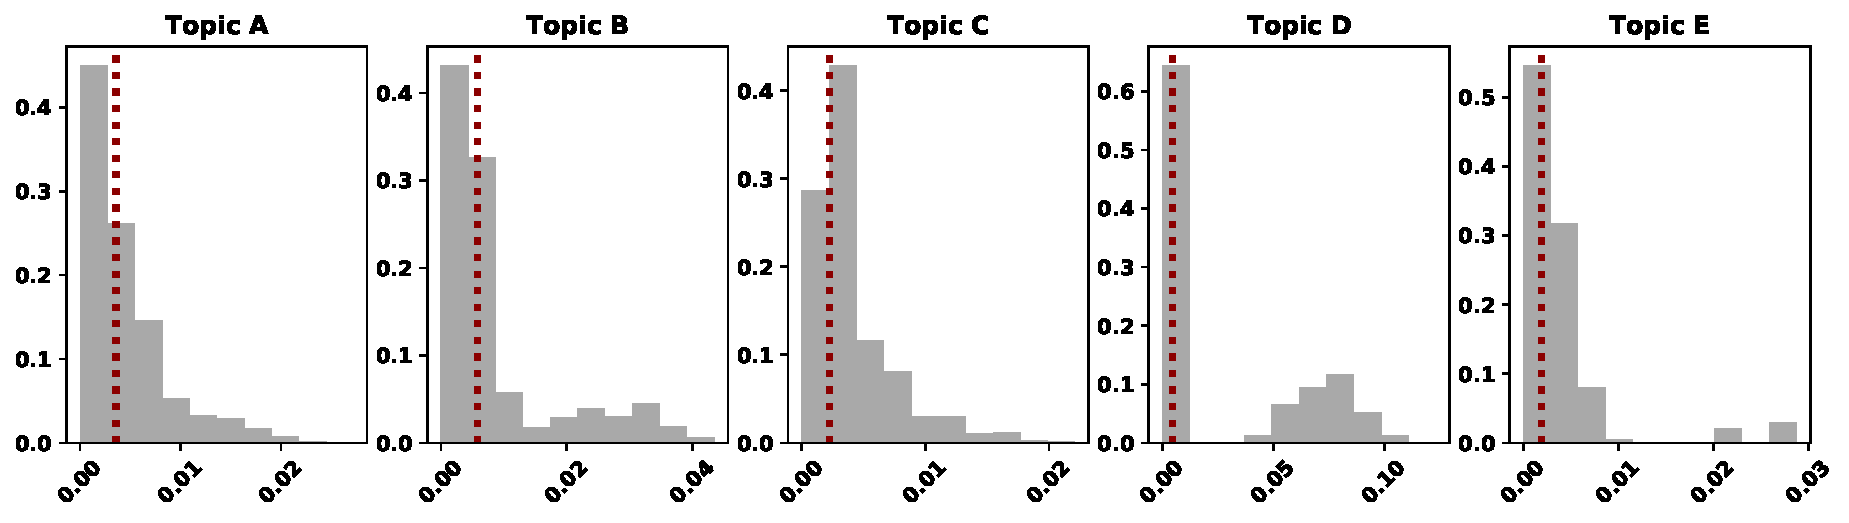
\includegraphics[width=\textwidth]{src/chapters/03/paper/bibliometric-study-of-the-prisoners-dilemma/assets/images/topics_closeness_distributions.pdf}
    \caption{Distributions of closeness centrality in topics' networks.}
    \label{fig:cc_distributions_topics}
\end{figure}
\end{appendices}

\end{document}
